% Options for packages loaded elsewhere
\PassOptionsToPackage{unicode}{hyperref}
\PassOptionsToPackage{hyphens}{url}
\PassOptionsToPackage{dvipsnames,svgnames,x11names}{xcolor}
%
\documentclass[
  letterpaper,
  DIV=11,
  numbers=noendperiod]{scrartcl}

\usepackage{amsmath,amssymb}
\usepackage{iftex}
\ifPDFTeX
  \usepackage[T1]{fontenc}
  \usepackage[utf8]{inputenc}
  \usepackage{textcomp} % provide euro and other symbols
\else % if luatex or xetex
  \usepackage{unicode-math}
  \defaultfontfeatures{Scale=MatchLowercase}
  \defaultfontfeatures[\rmfamily]{Ligatures=TeX,Scale=1}
\fi
\usepackage{lmodern}
\ifPDFTeX\else  
    % xetex/luatex font selection
\fi
% Use upquote if available, for straight quotes in verbatim environments
\IfFileExists{upquote.sty}{\usepackage{upquote}}{}
\IfFileExists{microtype.sty}{% use microtype if available
  \usepackage[]{microtype}
  \UseMicrotypeSet[protrusion]{basicmath} % disable protrusion for tt fonts
}{}
\makeatletter
\@ifundefined{KOMAClassName}{% if non-KOMA class
  \IfFileExists{parskip.sty}{%
    \usepackage{parskip}
  }{% else
    \setlength{\parindent}{0pt}
    \setlength{\parskip}{6pt plus 2pt minus 1pt}}
}{% if KOMA class
  \KOMAoptions{parskip=half}}
\makeatother
\usepackage{xcolor}
\usepackage[margin=1in]{geometry}
\setlength{\emergencystretch}{3em} % prevent overfull lines
\setcounter{secnumdepth}{5}
% Make \paragraph and \subparagraph free-standing
\makeatletter
\ifx\paragraph\undefined\else
  \let\oldparagraph\paragraph
  \renewcommand{\paragraph}{
    \@ifstar
      \xxxParagraphStar
      \xxxParagraphNoStar
  }
  \newcommand{\xxxParagraphStar}[1]{\oldparagraph*{#1}\mbox{}}
  \newcommand{\xxxParagraphNoStar}[1]{\oldparagraph{#1}\mbox{}}
\fi
\ifx\subparagraph\undefined\else
  \let\oldsubparagraph\subparagraph
  \renewcommand{\subparagraph}{
    \@ifstar
      \xxxSubParagraphStar
      \xxxSubParagraphNoStar
  }
  \newcommand{\xxxSubParagraphStar}[1]{\oldsubparagraph*{#1}\mbox{}}
  \newcommand{\xxxSubParagraphNoStar}[1]{\oldsubparagraph{#1}\mbox{}}
\fi
\makeatother

\usepackage{color}
\usepackage{fancyvrb}
\newcommand{\VerbBar}{|}
\newcommand{\VERB}{\Verb[commandchars=\\\{\}]}
\DefineVerbatimEnvironment{Highlighting}{Verbatim}{commandchars=\\\{\}}
% Add ',fontsize=\small' for more characters per line
\usepackage{framed}
\definecolor{shadecolor}{RGB}{241,243,245}
\newenvironment{Shaded}{\begin{snugshade}}{\end{snugshade}}
\newcommand{\AlertTok}[1]{\textcolor[rgb]{0.68,0.00,0.00}{#1}}
\newcommand{\AnnotationTok}[1]{\textcolor[rgb]{0.37,0.37,0.37}{#1}}
\newcommand{\AttributeTok}[1]{\textcolor[rgb]{0.40,0.45,0.13}{#1}}
\newcommand{\BaseNTok}[1]{\textcolor[rgb]{0.68,0.00,0.00}{#1}}
\newcommand{\BuiltInTok}[1]{\textcolor[rgb]{0.00,0.23,0.31}{#1}}
\newcommand{\CharTok}[1]{\textcolor[rgb]{0.13,0.47,0.30}{#1}}
\newcommand{\CommentTok}[1]{\textcolor[rgb]{0.37,0.37,0.37}{#1}}
\newcommand{\CommentVarTok}[1]{\textcolor[rgb]{0.37,0.37,0.37}{\textit{#1}}}
\newcommand{\ConstantTok}[1]{\textcolor[rgb]{0.56,0.35,0.01}{#1}}
\newcommand{\ControlFlowTok}[1]{\textcolor[rgb]{0.00,0.23,0.31}{\textbf{#1}}}
\newcommand{\DataTypeTok}[1]{\textcolor[rgb]{0.68,0.00,0.00}{#1}}
\newcommand{\DecValTok}[1]{\textcolor[rgb]{0.68,0.00,0.00}{#1}}
\newcommand{\DocumentationTok}[1]{\textcolor[rgb]{0.37,0.37,0.37}{\textit{#1}}}
\newcommand{\ErrorTok}[1]{\textcolor[rgb]{0.68,0.00,0.00}{#1}}
\newcommand{\ExtensionTok}[1]{\textcolor[rgb]{0.00,0.23,0.31}{#1}}
\newcommand{\FloatTok}[1]{\textcolor[rgb]{0.68,0.00,0.00}{#1}}
\newcommand{\FunctionTok}[1]{\textcolor[rgb]{0.28,0.35,0.67}{#1}}
\newcommand{\ImportTok}[1]{\textcolor[rgb]{0.00,0.46,0.62}{#1}}
\newcommand{\InformationTok}[1]{\textcolor[rgb]{0.37,0.37,0.37}{#1}}
\newcommand{\KeywordTok}[1]{\textcolor[rgb]{0.00,0.23,0.31}{\textbf{#1}}}
\newcommand{\NormalTok}[1]{\textcolor[rgb]{0.00,0.23,0.31}{#1}}
\newcommand{\OperatorTok}[1]{\textcolor[rgb]{0.37,0.37,0.37}{#1}}
\newcommand{\OtherTok}[1]{\textcolor[rgb]{0.00,0.23,0.31}{#1}}
\newcommand{\PreprocessorTok}[1]{\textcolor[rgb]{0.68,0.00,0.00}{#1}}
\newcommand{\RegionMarkerTok}[1]{\textcolor[rgb]{0.00,0.23,0.31}{#1}}
\newcommand{\SpecialCharTok}[1]{\textcolor[rgb]{0.37,0.37,0.37}{#1}}
\newcommand{\SpecialStringTok}[1]{\textcolor[rgb]{0.13,0.47,0.30}{#1}}
\newcommand{\StringTok}[1]{\textcolor[rgb]{0.13,0.47,0.30}{#1}}
\newcommand{\VariableTok}[1]{\textcolor[rgb]{0.07,0.07,0.07}{#1}}
\newcommand{\VerbatimStringTok}[1]{\textcolor[rgb]{0.13,0.47,0.30}{#1}}
\newcommand{\WarningTok}[1]{\textcolor[rgb]{0.37,0.37,0.37}{\textit{#1}}}

\providecommand{\tightlist}{%
  \setlength{\itemsep}{0pt}\setlength{\parskip}{0pt}}\usepackage{longtable,booktabs,array}
\usepackage{calc} % for calculating minipage widths
% Correct order of tables after \paragraph or \subparagraph
\usepackage{etoolbox}
\makeatletter
\patchcmd\longtable{\par}{\if@noskipsec\mbox{}\fi\par}{}{}
\makeatother
% Allow footnotes in longtable head/foot
\IfFileExists{footnotehyper.sty}{\usepackage{footnotehyper}}{\usepackage{footnote}}
\makesavenoteenv{longtable}
\usepackage{graphicx}
\makeatletter
\def\maxwidth{\ifdim\Gin@nat@width>\linewidth\linewidth\else\Gin@nat@width\fi}
\def\maxheight{\ifdim\Gin@nat@height>\textheight\textheight\else\Gin@nat@height\fi}
\makeatother
% Scale images if necessary, so that they will not overflow the page
% margins by default, and it is still possible to overwrite the defaults
% using explicit options in \includegraphics[width, height, ...]{}
\setkeys{Gin}{width=\maxwidth,height=\maxheight,keepaspectratio}
% Set default figure placement to htbp
\makeatletter
\def\fps@figure{htbp}
\makeatother

\KOMAoption{captions}{tableheading,figureheading}
\makeatletter
\@ifpackageloaded{caption}{}{\usepackage{caption}}
\AtBeginDocument{%
\ifdefined\contentsname
  \renewcommand*\contentsname{Table of contents}
\else
  \newcommand\contentsname{Table of contents}
\fi
\ifdefined\listfigurename
  \renewcommand*\listfigurename{List of Figures}
\else
  \newcommand\listfigurename{List of Figures}
\fi
\ifdefined\listtablename
  \renewcommand*\listtablename{List of Tables}
\else
  \newcommand\listtablename{List of Tables}
\fi
\ifdefined\figurename
  \renewcommand*\figurename{Figure}
\else
  \newcommand\figurename{Figure}
\fi
\ifdefined\tablename
  \renewcommand*\tablename{Table}
\else
  \newcommand\tablename{Table}
\fi
}
\@ifpackageloaded{float}{}{\usepackage{float}}
\floatstyle{ruled}
\@ifundefined{c@chapter}{\newfloat{codelisting}{h}{lop}}{\newfloat{codelisting}{h}{lop}[chapter]}
\floatname{codelisting}{Listing}
\newcommand*\listoflistings{\listof{codelisting}{List of Listings}}
\makeatother
\makeatletter
\makeatother
\makeatletter
\@ifpackageloaded{caption}{}{\usepackage{caption}}
\@ifpackageloaded{subcaption}{}{\usepackage{subcaption}}
\makeatother

\ifLuaTeX
  \usepackage{selnolig}  % disable illegal ligatures
\fi
\usepackage{bookmark}

\IfFileExists{xurl.sty}{\usepackage{xurl}}{} % add URL line breaks if available
\urlstyle{same} % disable monospaced font for URLs
\hypersetup{
  pdftitle={Polynomial Regression for ARC Adjustment},
  pdfauthor={Abdullah Azzam},
  colorlinks=true,
  linkcolor={blue},
  filecolor={Maroon},
  citecolor={Blue},
  urlcolor={Blue},
  pdfcreator={LaTeX via pandoc}}


\title{Polynomial Regression for ARC Adjustment}
\author{Abdullah Azzam}
\date{2025-07-01}

\begin{document}
\maketitle

\renewcommand*\contentsname{Table of contents}
{
\hypersetup{linkcolor=}
\setcounter{tocdepth}{3}
\tableofcontents
}

\section{Relationship between ARC II and ARCs I and
III}\label{relationship-between-arc-ii-and-arcs-i-and-iii}

\subsection{Data}\label{data}

Table 10-1 as dataframe

\begin{Shaded}
\begin{Highlighting}[]
\CommentTok{\# ARC II values}
\NormalTok{arc\_ii }\OtherTok{\textless{}{-}} \FunctionTok{c}\NormalTok{(}\DecValTok{100}\SpecialCharTok{:}\DecValTok{61}\NormalTok{, }\DecValTok{60}\SpecialCharTok{:}\DecValTok{30}\NormalTok{, }\DecValTok{25}\NormalTok{, }\DecValTok{20}\NormalTok{, }\DecValTok{15}\NormalTok{, }\DecValTok{10}\NormalTok{, }\DecValTok{5}\NormalTok{, }\DecValTok{0}\NormalTok{)}

\CommentTok{\# Corresponding ARC I values}
\NormalTok{arc\_i }\OtherTok{\textless{}{-}} \FunctionTok{c}\NormalTok{(}
  \DecValTok{100}\NormalTok{, }\DecValTok{97}\NormalTok{, }\DecValTok{94}\NormalTok{, }\DecValTok{91}\NormalTok{, }\DecValTok{89}\NormalTok{, }\DecValTok{87}\NormalTok{, }\DecValTok{85}\NormalTok{, }\DecValTok{83}\NormalTok{, }\DecValTok{81}\NormalTok{, }\DecValTok{80}\NormalTok{,}
   \DecValTok{78}\NormalTok{, }\DecValTok{76}\NormalTok{, }\DecValTok{75}\NormalTok{, }\DecValTok{73}\NormalTok{, }\DecValTok{72}\NormalTok{, }\DecValTok{70}\NormalTok{, }\DecValTok{68}\NormalTok{, }\DecValTok{67}\NormalTok{, }\DecValTok{66}\NormalTok{, }\DecValTok{64}\NormalTok{,}
   \DecValTok{63}\NormalTok{, }\DecValTok{62}\NormalTok{, }\DecValTok{60}\NormalTok{, }\DecValTok{59}\NormalTok{, }\DecValTok{58}\NormalTok{, }\DecValTok{57}\NormalTok{, }\DecValTok{55}\NormalTok{, }\DecValTok{54}\NormalTok{, }\DecValTok{53}\NormalTok{, }\DecValTok{52}\NormalTok{,}
   \DecValTok{51}\NormalTok{, }\DecValTok{50}\NormalTok{, }\DecValTok{48}\NormalTok{, }\DecValTok{47}\NormalTok{, }\DecValTok{46}\NormalTok{, }\DecValTok{45}\NormalTok{, }\DecValTok{44}\NormalTok{, }\DecValTok{43}\NormalTok{, }\DecValTok{42}\NormalTok{, }\DecValTok{41}\NormalTok{,}
   \DecValTok{40}\NormalTok{, }\DecValTok{39}\NormalTok{, }\DecValTok{38}\NormalTok{, }\DecValTok{37}\NormalTok{, }\DecValTok{36}\NormalTok{, }\DecValTok{35}\NormalTok{, }\DecValTok{34}\NormalTok{, }\DecValTok{33}\NormalTok{, }\DecValTok{32}\NormalTok{, }\DecValTok{31}\NormalTok{,}
   \DecValTok{31}\NormalTok{, }\DecValTok{30}\NormalTok{, }\DecValTok{29}\NormalTok{, }\DecValTok{28}\NormalTok{, }\DecValTok{27}\NormalTok{, }\DecValTok{26}\NormalTok{, }\DecValTok{25}\NormalTok{, }\DecValTok{25}\NormalTok{, }\DecValTok{24}\NormalTok{, }\DecValTok{23}\NormalTok{,}
   \DecValTok{22}\NormalTok{, }\DecValTok{21}\NormalTok{, }\DecValTok{21}\NormalTok{, }\DecValTok{20}\NormalTok{, }\DecValTok{19}\NormalTok{, }\DecValTok{18}\NormalTok{, }\DecValTok{18}\NormalTok{, }\DecValTok{17}\NormalTok{, }\DecValTok{16}\NormalTok{, }\DecValTok{16}\NormalTok{,}
   \DecValTok{15}\NormalTok{, }\DecValTok{12}\NormalTok{,  }\DecValTok{9}\NormalTok{,  }\DecValTok{6}\NormalTok{,  }\DecValTok{4}\NormalTok{,  }\DecValTok{2}\NormalTok{,  }\DecValTok{0}
\NormalTok{)}

\CommentTok{\# Corresponding ARC III values}
\NormalTok{arc\_iii }\OtherTok{\textless{}{-}} \FunctionTok{c}\NormalTok{(}
  \DecValTok{100}\NormalTok{,}\DecValTok{100}\NormalTok{, }\DecValTok{99}\NormalTok{, }\DecValTok{99}\NormalTok{, }\DecValTok{99}\NormalTok{, }\DecValTok{98}\NormalTok{, }\DecValTok{98}\NormalTok{, }\DecValTok{98}\NormalTok{, }\DecValTok{97}\NormalTok{, }\DecValTok{97}\NormalTok{,}
   \DecValTok{96}\NormalTok{, }\DecValTok{96}\NormalTok{, }\DecValTok{95}\NormalTok{, }\DecValTok{95}\NormalTok{, }\DecValTok{94}\NormalTok{, }\DecValTok{94}\NormalTok{, }\DecValTok{93}\NormalTok{, }\DecValTok{93}\NormalTok{, }\DecValTok{92}\NormalTok{, }\DecValTok{92}\NormalTok{,}
   \DecValTok{91}\NormalTok{, }\DecValTok{91}\NormalTok{, }\DecValTok{90}\NormalTok{, }\DecValTok{89}\NormalTok{, }\DecValTok{89}\NormalTok{, }\DecValTok{88}\NormalTok{, }\DecValTok{88}\NormalTok{, }\DecValTok{87}\NormalTok{, }\DecValTok{86}\NormalTok{, }\DecValTok{86}\NormalTok{,}
   \DecValTok{85}\NormalTok{, }\DecValTok{84}\NormalTok{, }\DecValTok{84}\NormalTok{, }\DecValTok{83}\NormalTok{, }\DecValTok{82}\NormalTok{, }\DecValTok{82}\NormalTok{, }\DecValTok{81}\NormalTok{, }\DecValTok{80}\NormalTok{, }\DecValTok{79}\NormalTok{, }\DecValTok{78}\NormalTok{,}
   \DecValTok{78}\NormalTok{, }\DecValTok{77}\NormalTok{, }\DecValTok{76}\NormalTok{, }\DecValTok{75}\NormalTok{, }\DecValTok{75}\NormalTok{, }\DecValTok{74}\NormalTok{, }\DecValTok{73}\NormalTok{, }\DecValTok{72}\NormalTok{, }\DecValTok{71}\NormalTok{, }\DecValTok{70}\NormalTok{,}
   \DecValTok{70}\NormalTok{, }\DecValTok{69}\NormalTok{, }\DecValTok{68}\NormalTok{, }\DecValTok{67}\NormalTok{, }\DecValTok{66}\NormalTok{, }\DecValTok{65}\NormalTok{, }\DecValTok{64}\NormalTok{, }\DecValTok{63}\NormalTok{, }\DecValTok{62}\NormalTok{, }\DecValTok{61}\NormalTok{,}
   \DecValTok{60}\NormalTok{, }\DecValTok{59}\NormalTok{, }\DecValTok{58}\NormalTok{, }\DecValTok{57}\NormalTok{, }\DecValTok{56}\NormalTok{, }\DecValTok{55}\NormalTok{, }\DecValTok{54}\NormalTok{, }\DecValTok{53}\NormalTok{, }\DecValTok{52}\NormalTok{, }\DecValTok{51}\NormalTok{,}
   \DecValTok{50}\NormalTok{, }\DecValTok{43}\NormalTok{, }\DecValTok{37}\NormalTok{, }\DecValTok{30}\NormalTok{, }\DecValTok{22}\NormalTok{, }\DecValTok{13}\NormalTok{,  }\DecValTok{0}
\NormalTok{)}

\NormalTok{df\_cn }\OtherTok{\textless{}{-}} \FunctionTok{data.frame}\NormalTok{(}
  \AttributeTok{arc\_ii =}\NormalTok{ arc\_ii,}
  \AttributeTok{arc\_i =}\NormalTok{ arc\_i,}
  \AttributeTok{arc\_iii =}\NormalTok{ arc\_iii}
\NormalTok{)}

\CommentTok{\# quick check}
\FunctionTok{head}\NormalTok{(df\_cn, }\DecValTok{10}\NormalTok{)}
\end{Highlighting}
\end{Shaded}

\begin{verbatim}
   arc_ii arc_i arc_iii
1     100   100     100
2      99    97     100
3      98    94      99
4      97    91      99
5      96    89      99
6      95    87      98
7      94    85      98
8      93    83      98
9      92    81      97
10     91    80      97
\end{verbatim}

\subsection{linear models: arc ii vs i, and ii vs
iii}\label{linear-models-arc-ii-vs-i-and-ii-vs-iii}

Let's try the simplest model (linear):

\[
\begin{aligned}
\mathrm{ARC\ I}   &= \alpha_{1} + \beta_{1}\,(\mathrm{ARC\ II}), \\
\mathrm{ARC\ III} &= \alpha_{3} + \beta_{3}\,(\mathrm{ARC\ II}).
\end{aligned}
\]

\begin{Shaded}
\begin{Highlighting}[]
\NormalTok{mod\_i   }\OtherTok{\textless{}{-}} \FunctionTok{lm}\NormalTok{(arc\_i   }\SpecialCharTok{\textasciitilde{}}\NormalTok{ arc\_ii,  }\AttributeTok{data =}\NormalTok{ df\_cn)}
\NormalTok{mod\_iii }\OtherTok{\textless{}{-}} \FunctionTok{lm}\NormalTok{(arc\_iii }\SpecialCharTok{\textasciitilde{}}\NormalTok{ arc\_ii,  }\AttributeTok{data =}\NormalTok{ df\_cn)}

\NormalTok{ci }\OtherTok{\textless{}{-}} \FunctionTok{coef}\NormalTok{(mod\_i)}
\NormalTok{c3 }\OtherTok{\textless{}{-}} \FunctionTok{coef}\NormalTok{(mod\_iii)}

\FunctionTok{cat}\NormalTok{(}\StringTok{"ARC I ="}\NormalTok{, }\FunctionTok{round}\NormalTok{(ci[}\DecValTok{2}\NormalTok{],}\DecValTok{4}\NormalTok{), }\StringTok{"* ARC II"}\NormalTok{, }\ControlFlowTok{if}\NormalTok{(ci[}\DecValTok{1}\NormalTok{]}\SpecialCharTok{\textgreater{}=}\DecValTok{0}\NormalTok{) }\StringTok{"+"} \ControlFlowTok{else} \StringTok{"{-}"}\NormalTok{, }\FunctionTok{abs}\NormalTok{(}\FunctionTok{round}\NormalTok{(ci[}\DecValTok{1}\NormalTok{],}\DecValTok{4}\NormalTok{)), }\StringTok{"}\SpecialCharTok{\textbackslash{}n}\StringTok{"}\NormalTok{)}
\end{Highlighting}
\end{Shaded}

\begin{verbatim}
ARC I = 1.0243 * ARC II - 17.1276 
\end{verbatim}

\begin{Shaded}
\begin{Highlighting}[]
\FunctionTok{cat}\NormalTok{(}\StringTok{"ARC III ="}\NormalTok{, }\FunctionTok{round}\NormalTok{(c3[}\DecValTok{2}\NormalTok{],}\DecValTok{4}\NormalTok{), }\StringTok{"* ARC II"}\NormalTok{, }\ControlFlowTok{if}\NormalTok{(c3[}\DecValTok{1}\NormalTok{]}\SpecialCharTok{\textgreater{}=}\DecValTok{0}\NormalTok{) }\StringTok{"+"} \ControlFlowTok{else} \StringTok{"{-}"}\NormalTok{, }\FunctionTok{abs}\NormalTok{(}\FunctionTok{round}\NormalTok{(c3[}\DecValTok{1}\NormalTok{],}\DecValTok{4}\NormalTok{)), }\StringTok{"}\SpecialCharTok{\textbackslash{}n}\StringTok{"}\NormalTok{)}
\end{Highlighting}
\end{Shaded}

\begin{verbatim}
ARC III = 0.8403 * ARC II + 23.8025 
\end{verbatim}

\begin{Shaded}
\begin{Highlighting}[]
\FunctionTok{par}\NormalTok{(}\AttributeTok{mfrow=}\FunctionTok{c}\NormalTok{(}\DecValTok{1}\NormalTok{,}\DecValTok{2}\NormalTok{), }\AttributeTok{mar=}\FunctionTok{c}\NormalTok{(}\DecValTok{4}\NormalTok{,}\DecValTok{4}\NormalTok{,}\DecValTok{2}\NormalTok{,}\DecValTok{1}\NormalTok{))}
\FunctionTok{plot}\NormalTok{(df\_cn}\SpecialCharTok{$}\NormalTok{arc\_ii, df\_cn}\SpecialCharTok{$}\NormalTok{arc\_i,   }\AttributeTok{main=}\StringTok{"ARC I vs ARC II"}\NormalTok{,}
     \AttributeTok{xlab=}\StringTok{"ARC II"}\NormalTok{, }\AttributeTok{ylab=}\StringTok{"ARC I"}\NormalTok{);   }\FunctionTok{abline}\NormalTok{(mod\_i)}
\FunctionTok{plot}\NormalTok{(df\_cn}\SpecialCharTok{$}\NormalTok{arc\_ii, df\_cn}\SpecialCharTok{$}\NormalTok{arc\_iii, }\AttributeTok{main=}\StringTok{"ARC III vs ARC II"}\NormalTok{,}
     \AttributeTok{xlab=}\StringTok{"ARC II"}\NormalTok{, }\AttributeTok{ylab=}\StringTok{"ARC III"}\NormalTok{); }\FunctionTok{abline}\NormalTok{(mod\_iii)}
\end{Highlighting}
\end{Shaded}

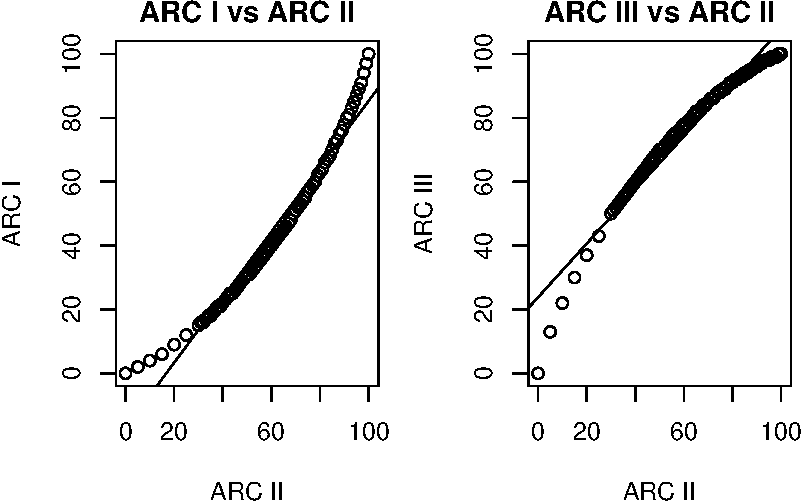
\includegraphics{arc_conversion_files/figure-pdf/unnamed-chunk-2-1.pdf}

\subsection{Polynomial Regression}\label{polynomial-regression}

Fit raw-power polynomials of degree ( d = 1 \dots 4 ):

\[
\text{ARC I}(x) = \beta_0 + \beta_1 x + \beta_2 x^2 + \beta_3 x^3 + \beta_4 x^4,
\]

\[
\text{ARC III}(x) = \gamma_0 + \gamma_1 x + \gamma_2 x^2 + \gamma_3 x^3 + \gamma_4 x^4,
\]

where ( x = \text{ARC II} ). Select the best ( d ) by minimizing AIC.

\begin{Shaded}
\begin{Highlighting}[]
\NormalTok{fit\_and\_evaluate }\OtherTok{\textless{}{-}} \ControlFlowTok{function}\NormalTok{(y, x, }\AttributeTok{max\_deg=}\DecValTok{4}\NormalTok{, data)\{}
\NormalTok{  fits }\OtherTok{\textless{}{-}} \FunctionTok{lapply}\NormalTok{(}\DecValTok{1}\SpecialCharTok{:}\NormalTok{max\_deg, }\ControlFlowTok{function}\NormalTok{(d)\{}
    \FunctionTok{lm}\NormalTok{(}\FunctionTok{as.formula}\NormalTok{(}\FunctionTok{sprintf}\NormalTok{(}\StringTok{"\%s \textasciitilde{} poly(\%s,\%d,raw=TRUE)"}\NormalTok{, y, x, d)), }\AttributeTok{data=}\NormalTok{data)}
\NormalTok{  \})}
\NormalTok{  metrics }\OtherTok{\textless{}{-}} \FunctionTok{data.frame}\NormalTok{(}
    \AttributeTok{degree =} \DecValTok{1}\SpecialCharTok{:}\DecValTok{4}\NormalTok{,}
    \AttributeTok{AIC    =} \FunctionTok{sapply}\NormalTok{(fits, AIC),}
    \AttributeTok{adj\_R2 =} \FunctionTok{sapply}\NormalTok{(fits, }\ControlFlowTok{function}\NormalTok{(m) }\FunctionTok{summary}\NormalTok{(m)}\SpecialCharTok{$}\NormalTok{adj.r.squared)}
\NormalTok{  )}
\NormalTok{  best }\OtherTok{\textless{}{-}}\NormalTok{ metrics}\SpecialCharTok{$}\NormalTok{degree[}\FunctionTok{which.min}\NormalTok{(metrics}\SpecialCharTok{$}\NormalTok{AIC)]}
  \FunctionTok{list}\NormalTok{(}\AttributeTok{metrics=}\NormalTok{metrics, }\AttributeTok{best=}\NormalTok{best, }\AttributeTok{fit=}\NormalTok{fits[[best]])}
\NormalTok{\}}

\NormalTok{res\_i   }\OtherTok{\textless{}{-}} \FunctionTok{fit\_and\_evaluate}\NormalTok{(}\StringTok{"arc\_i"}\NormalTok{,   }\StringTok{"arc\_ii"}\NormalTok{, }\AttributeTok{data=}\NormalTok{df\_cn)}
\NormalTok{res\_iii }\OtherTok{\textless{}{-}} \FunctionTok{fit\_and\_evaluate}\NormalTok{(}\StringTok{"arc\_iii"}\NormalTok{, }\StringTok{"arc\_ii"}\NormalTok{, }\AttributeTok{data=}\NormalTok{df\_cn)}

\NormalTok{res\_i}\SpecialCharTok{$}\NormalTok{metrics}
\end{Highlighting}
\end{Shaded}

\begin{verbatim}
  degree      AIC    adj_R2
1      1 476.8652 0.9584608
2      2 252.4888 0.9977742
3      3 174.7730 0.9991987
4      4 109.2585 0.9996620
\end{verbatim}

\begin{Shaded}
\begin{Highlighting}[]
\NormalTok{res\_iii}\SpecialCharTok{$}\NormalTok{metrics}
\end{Highlighting}
\end{Shaded}

\begin{verbatim}
  degree       AIC    adj_R2
1      1 463.94746 0.9483609
2      2 217.60273 0.9979198
3      3 143.34330 0.9992168
4      4  75.66948 0.9996787
\end{verbatim}

\begin{Shaded}
\begin{Highlighting}[]
\FunctionTok{cat}\NormalTok{(}\StringTok{"Best degree for ARC I   ="}\NormalTok{, res\_i}\SpecialCharTok{$}\NormalTok{best,   }\StringTok{"}\SpecialCharTok{\textbackslash{}n}\StringTok{"}\NormalTok{)}
\end{Highlighting}
\end{Shaded}

\begin{verbatim}
Best degree for ARC I   = 4 
\end{verbatim}

\begin{Shaded}
\begin{Highlighting}[]
\FunctionTok{cat}\NormalTok{(}\StringTok{"Best degree for ARC III ="}\NormalTok{, res\_iii}\SpecialCharTok{$}\NormalTok{best, }\StringTok{"}\SpecialCharTok{\textbackslash{}n}\StringTok{"}\NormalTok{)}
\end{Highlighting}
\end{Shaded}

\begin{verbatim}
Best degree for ARC III = 4 
\end{verbatim}

\begin{Shaded}
\begin{Highlighting}[]
\NormalTok{xx }\OtherTok{\textless{}{-}} \FunctionTok{seq}\NormalTok{(}\DecValTok{0}\NormalTok{,}\DecValTok{100}\NormalTok{,}\AttributeTok{length=}\DecValTok{200}\NormalTok{)}
\FunctionTok{par}\NormalTok{(}\AttributeTok{mfrow=}\FunctionTok{c}\NormalTok{(}\DecValTok{1}\NormalTok{,}\DecValTok{2}\NormalTok{), }\AttributeTok{mar=}\FunctionTok{c}\NormalTok{(}\DecValTok{4}\NormalTok{,}\DecValTok{4}\NormalTok{,}\DecValTok{2}\NormalTok{,}\DecValTok{1}\NormalTok{))}
\FunctionTok{plot}\NormalTok{(df\_cn}\SpecialCharTok{$}\NormalTok{arc\_ii, df\_cn}\SpecialCharTok{$}\NormalTok{arc\_i, }\AttributeTok{main=}\StringTok{"Poly Fit: ARC I"}\NormalTok{)}
\FunctionTok{lines}\NormalTok{(xx, }\FunctionTok{predict}\NormalTok{(res\_i}\SpecialCharTok{$}\NormalTok{fit,   }\AttributeTok{newdata=}\FunctionTok{data.frame}\NormalTok{(}\AttributeTok{arc\_ii=}\NormalTok{xx)), }\AttributeTok{lwd=}\DecValTok{2}\NormalTok{)}
\FunctionTok{plot}\NormalTok{(df\_cn}\SpecialCharTok{$}\NormalTok{arc\_ii, df\_cn}\SpecialCharTok{$}\NormalTok{arc\_iii, }\AttributeTok{main=}\StringTok{"Poly Fit: ARC III"}\NormalTok{)}
\FunctionTok{lines}\NormalTok{(xx, }\FunctionTok{predict}\NormalTok{(res\_iii}\SpecialCharTok{$}\NormalTok{fit, }\AttributeTok{newdata=}\FunctionTok{data.frame}\NormalTok{(}\AttributeTok{arc\_ii=}\NormalTok{xx)), }\AttributeTok{lwd=}\DecValTok{2}\NormalTok{)}
\end{Highlighting}
\end{Shaded}

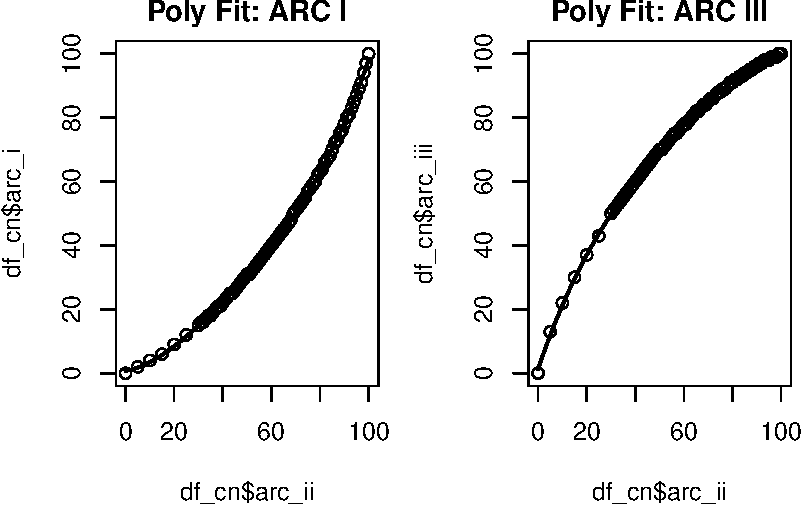
\includegraphics{arc_conversion_files/figure-pdf/unnamed-chunk-3-1.pdf}

\subsection{Final Degree-4 Equations}\label{final-degree-4-equations}

A 4th-degree polynomial minimizes AIC in both cases. Extracting and
ordering the coefficients gives:

\[
\text{ARC I}(x) = 1.2211 \times 10^{-6} x^4 - 2.0260 \times 10^{-4} x^3 + 1.6526 \times 10^{-2} x^2 + 0.12577 x + 0.74712,
\]

\[
\text{ARC III}(x) = -1.0054 \times 10^{-6} x^4 + 2.5082 \times 10^{-4} x^3 - 2.7615 \times 10^{-2} x^2 + 2.24312 x + 1.30209.
\]

\begin{Shaded}
\begin{Highlighting}[]
\NormalTok{mod\_i4   }\OtherTok{\textless{}{-}} \FunctionTok{lm}\NormalTok{(arc\_i   }\SpecialCharTok{\textasciitilde{}}\NormalTok{ arc\_ii }\SpecialCharTok{+} \FunctionTok{I}\NormalTok{(arc\_ii}\SpecialCharTok{\^{}}\DecValTok{2}\NormalTok{) }\SpecialCharTok{+} \FunctionTok{I}\NormalTok{(arc\_ii}\SpecialCharTok{\^{}}\DecValTok{3}\NormalTok{) }\SpecialCharTok{+} \FunctionTok{I}\NormalTok{(arc\_ii}\SpecialCharTok{\^{}}\DecValTok{4}\NormalTok{), df\_cn)}
\NormalTok{mod\_iii4 }\OtherTok{\textless{}{-}} \FunctionTok{lm}\NormalTok{(arc\_iii }\SpecialCharTok{\textasciitilde{}}\NormalTok{ arc\_ii }\SpecialCharTok{+} \FunctionTok{I}\NormalTok{(arc\_ii}\SpecialCharTok{\^{}}\DecValTok{2}\NormalTok{) }\SpecialCharTok{+} \FunctionTok{I}\NormalTok{(arc\_ii}\SpecialCharTok{\^{}}\DecValTok{3}\NormalTok{) }\SpecialCharTok{+} \FunctionTok{I}\NormalTok{(arc\_ii}\SpecialCharTok{\^{}}\DecValTok{4}\NormalTok{), df\_cn)}

\NormalTok{poly\_i   }\OtherTok{\textless{}{-}} \FunctionTok{coef}\NormalTok{(mod\_i4)[}\FunctionTok{c}\NormalTok{(}\StringTok{"I(arc\_ii\^{}4)"}\NormalTok{,}\StringTok{"I(arc\_ii\^{}3)"}\NormalTok{,}\StringTok{"I(arc\_ii\^{}2)"}\NormalTok{,}\StringTok{"arc\_ii"}\NormalTok{,}\StringTok{"(Intercept)"}\NormalTok{)]}
\NormalTok{poly\_iii }\OtherTok{\textless{}{-}} \FunctionTok{coef}\NormalTok{(mod\_iii4)[}\FunctionTok{c}\NormalTok{(}\StringTok{"I(arc\_ii\^{}4)"}\NormalTok{,}\StringTok{"I(arc\_ii\^{}3)"}\NormalTok{,}\StringTok{"I(arc\_ii\^{}2)"}\NormalTok{,}\StringTok{"arc\_ii"}\NormalTok{,}\StringTok{"(Intercept)"}\NormalTok{)]}
\NormalTok{poly\_i}
\end{Highlighting}
\end{Shaded}

\begin{verbatim}
  I(arc_ii^4)   I(arc_ii^3)   I(arc_ii^2)        arc_ii   (Intercept) 
 1.221107e-06 -2.025995e-04  1.652565e-02  1.257686e-01  7.471240e-01 
\end{verbatim}

\begin{Shaded}
\begin{Highlighting}[]
\NormalTok{poly\_iii}
\end{Highlighting}
\end{Shaded}

\begin{verbatim}
  I(arc_ii^4)   I(arc_ii^3)   I(arc_ii^2)        arc_ii   (Intercept) 
-1.005440e-06  2.508244e-04 -2.761460e-02  2.243122e+00  1.302090e+00 
\end{verbatim}

\subsection{Using the conversion
function}\label{using-the-conversion-function}

\begin{Shaded}
\begin{Highlighting}[]
\NormalTok{predict\_arc\_i }\OtherTok{\textless{}{-}} \ControlFlowTok{function}\NormalTok{(x) \{}
  \FunctionTok{round}\NormalTok{((}\FunctionTok{sapply}\NormalTok{(x, }\ControlFlowTok{function}\NormalTok{(xi) }\FunctionTok{sum}\NormalTok{(poly\_i }\SpecialCharTok{*}\NormalTok{ xi}\SpecialCharTok{\^{}}\NormalTok{(}\DecValTok{4}\SpecialCharTok{:}\DecValTok{0}\NormalTok{)))),}\DecValTok{0}\NormalTok{)}
\CommentTok{\#  ceiling((sapply(x, function(xi) sum(poly\_i * xi\^{}(4:0)))))}
\NormalTok{\}}
\NormalTok{predict\_arc\_iii }\OtherTok{\textless{}{-}} \ControlFlowTok{function}\NormalTok{(x) \{}
  \FunctionTok{round}\NormalTok{((}\FunctionTok{sapply}\NormalTok{(x, }\ControlFlowTok{function}\NormalTok{(xi) }\FunctionTok{sum}\NormalTok{(poly\_iii}\SpecialCharTok{*}\NormalTok{ xi}\SpecialCharTok{\^{}}\NormalTok{(}\DecValTok{4}\SpecialCharTok{:}\DecValTok{0}\NormalTok{)))),}\DecValTok{0}\NormalTok{)}
\NormalTok{\}}
\CommentTok{\#predict\_arc\_i(c(30, 50, 75))}
\CommentTok{\#predict\_arc\_iii(c(30, 50, 75))}
\CommentTok{\#predict\_arc\_iii(c(72, 57, 88, 91, 45, 34, 66))}
\FunctionTok{predict\_arc\_i}\NormalTok{(}\FunctionTok{c}\NormalTok{(}\DecValTok{100}\NormalTok{, }\DecValTok{97}\NormalTok{, }\DecValTok{91}\NormalTok{, }\DecValTok{88}\NormalTok{, }\DecValTok{84}\NormalTok{, }\DecValTok{79}\NormalTok{, }\DecValTok{72}\NormalTok{, }\DecValTok{68}\NormalTok{, }\DecValTok{63}\NormalTok{, }\DecValTok{55}\NormalTok{, }\DecValTok{50}\NormalTok{, }\DecValTok{44}\NormalTok{, }\DecValTok{32}\NormalTok{))}
\end{Highlighting}
\end{Shaded}

\begin{verbatim}
 [1] 98 92 80 75 69 61 53 48 43 35 31 26 16
\end{verbatim}

\begin{Shaded}
\begin{Highlighting}[]
\FunctionTok{predict\_arc\_iii}\NormalTok{(}\FunctionTok{c}\NormalTok{(}\DecValTok{97}\NormalTok{, }\DecValTok{91}\NormalTok{, }\DecValTok{88}\NormalTok{, }\DecValTok{84}\NormalTok{, }\DecValTok{79}\NormalTok{, }\DecValTok{72}\NormalTok{, }\DecValTok{68}\NormalTok{, }\DecValTok{63}\NormalTok{, }\DecValTok{55}\NormalTok{, }\DecValTok{50}\NormalTok{, }\DecValTok{44}\NormalTok{, }\DecValTok{32}\NormalTok{))}
\end{Highlighting}
\end{Shaded}

\begin{verbatim}
 [1] 99 97 95 93 91 86 84 80 74 69 64 52
\end{verbatim}




\end{document}
